%!TEX program=pdflatex
\documentclass[8pt,xcolor={dvipsnames,table,xcdraw},handout]{beamer} % option aspectratio=169 for wide screen
\usetheme[
%%% options passed to the outer theme
    progressstyle=movCircCnt,   %either fixedCircCnt, movCircCnt, or corner
    rotationcw,          % change the rotation direction from counter-clockwise to clockwise
%    shownavsym          % show the navigation symbols
  ]{Cinvestav}
  
\usepackage[utf8]{inputenc}
\usepackage{csquotes}
\usepackage[english]{babel}
\usepackage[T1]{fontenc}
\usepackage{epigraph}
\usepackage{amsmath}
\usepackage{stmaryrd}
\usepackage[ruled]{algorithm2e}
\usepackage{caption}
\usepackage[absolute,overlay]{textpos}
\usepackage{hyperref}
\SetAlCapFnt{\small}
\SetAlCapNameFnt{\small}

\setbeamerfont{caption}{size=\scriptsize}
% colored hyperlinks
\newcommand{\chref}[2]{%
  \href{#1}{{\usebeamercolor[bg]{AAUsimple}#2}}%
}
\definecolor{sortOfBlueColor}{RGB}{0,200,255}
\newcommand{\markdone}{\textcolor{PineGreen}{$\bullet$}}
\newcommand{\markonprogress}{\textcolor{sortOfBlueColor}{$\bullet$}}
\newcommand{\markoff}{\textcolor{PineGreen}{$\circ$}}
\usepackage{booktabs}
\usepackage{makecell}
\usepackage{multicol}
\usepackage{multirow}
\usepackage{PTSans}


\title[Short thesis title]{Long, very long thesis title}
         
\author[ITL Cinvestav-Tamaulipas]{Student name}

\institute[
  ITL Information Technology Laboratory\\
  Cinvestav\\
  Tamaulipas
] 
{Advisor 1\\Advisor 2\\ITL Cinvestav}

\date{Reason of presentation, August 2017}

\graphicspath{ {images/} }

% Gain some extra space on slides
\setbeamersize{text margin left=5mm,text margin right=5mm} 

% Put a "separator" at the beginning of each section with the section title
% \AtBeginSection[]{
%   \begin{frame}
%   \vfill
%   \centering
%   \begin{beamercolorbox}[sep=8pt,center,shadow=true,rounded=true]{title}
%     \usebeamerfont{title}\insertsectionhead\par%
%   \end{beamercolorbox}
%   \vfill
%   \end{frame}
% }

\begin{document}
{\aauwavesbg%
\begin{frame}[plain,noframenumbering] % the plain option removes the header from the title page
  \titlepage
\end{frame}}

%!TEX root = slides.tex
\begin{frame}{Agenda}{}
\small
\tableofcontents
\end{frame}

%!TEX root = slides.tex
\section{Introduction}
\subsection{Motivation}
\begin{frame}{Research background}{Motivation}
\small
\begin{figure}[tb]
  \centering
  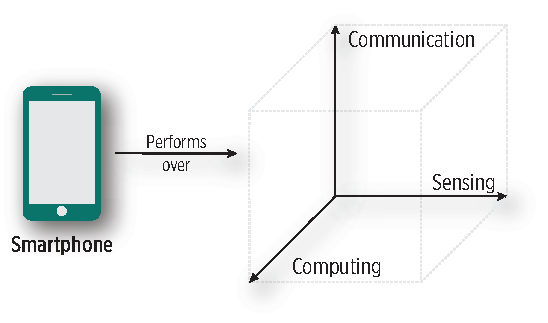
\includegraphics[width=0.4\textwidth]{smartphone-dimensions-for-thesis}
  \caption{Figure caption.}  
\end{figure}

\begin{block}{\small \textbf{Block title}}
  \begin{itemize}
  \item Text level 1 \cite{Berry2011}.
  \begin{itemize}
    \item Text level 2.
  \end{itemize}
\end{itemize}
\end{block}
\end{frame}

%!TEX root = slides.tex
\section{Future work}
\begin{frame}{Future work}{Pending tasks}
\begin{table}
%\renewcommand{\arraystretch}{1.2}
\centering
\resizebox{0.9\textwidth}{!}{%
\begin{tabular}{lllllllllllllll}
   &                                                                                                                             & \multicolumn{5}{c}{2017}                                                                                                                  & \multicolumn{8}{c}{2018}                                                                                                                                                                                                      \\
   \toprule
\# & \multicolumn{1}{c}{Activity}                                                                                                & \multicolumn{1}{c}{\scriptsize{Aug}}   & \multicolumn{1}{c}{\scriptsize{Sep}}   & \multicolumn{1}{c}{\scriptsize{Oct}}   & \multicolumn{1}{c}{\scriptsize{Nov}}   & \multicolumn{1}{c}{\scriptsize{Dec}}   & \multicolumn{1}{c}{\scriptsize{Jan}}   & \multicolumn{1}{c}{\scriptsize{Feb}}   & \multicolumn{1}{c}{\scriptsize{Mar}}   & \multicolumn{1}{c}{\scriptsize{Apr}}   & \multicolumn{1}{c}{\scriptsize{May}}   & \multicolumn{1}{c}{\scriptsize{Jun}}   & \multicolumn{1}{c}{\scriptsize{Jul}}   & \multicolumn{1}{c}{\scriptsize{Aug}}   \\
\midrule
\multicolumn{2}{c}{\textbf{Group 1}}                                                                               &                           &                           &                           &                           &                           &                           &                           &                           &                           &                           &                           &                           &                           \\
%\cmidrule{1-15}
1  & Activity 1                                                                                   & \cellcolor[HTML]{00D2CB} & \cellcolor[HTML]{00D2CB} &                           &                           &                           &                           &                           &                           &                           &                           &                           &                           &                           \\
\cmidrule[0.25pt]{1-15}
2  & \begin{tabular}[c]{@{}l@{}}Activity 2\end{tabular}                               &                           & \cellcolor[HTML]{00D2CB} & \cellcolor[HTML]{00D2CB} &                           &                           &                           &                           &                           &                           &                           &                           &                           &                           \\ 
\cmidrule[0.75pt]{1-15}
\multicolumn{2}{c}{\rule{0pt}{4ex}\textbf{Group two}}                                                                &                           &                           &                           &                           &                           &                           &                           &                           &                           &                           &                           &                           &                           \\
%\cmidrule{1-15}
3  & \rule{0pt}{2ex}Task 3                                                                                     &                           &                           &                           & \cellcolor[HTML]{00D2CB} &                           &                           &                           &                           &                           &                           &                           &                           &                           \\
\cmidrule[0.25pt]{1-15}
4  & \begin{tabular}[c]{@{}l@{}}Task 4\end{tabular}            &                           &                           &                           & \cellcolor[HTML]{00D2CB} &                           &                           &                           &                           &                           &                           &                           &                           &                           \\
\cmidrule[0.25pt]{1-15}
5  & \begin{tabular}[c]{@{}l@{}}Task 5\end{tabular} &                           &                           &                           & \cellcolor[HTML]{00D2CB} & \cellcolor[HTML]{00D2CB} &                           &                           &                           &                           &                           &                           &                           &                           \\
\cmidrule[0.5pt]{1-15}


\multicolumn{2}{c}{\rule{0pt}{4ex}\textbf{Group three}}                                                                &                           &                           &                           &                           &                           &                           &                           &                           &                           &                           &                           &                           &                           \\
6  & \begin{tabular}[c]{@{}l@{}}Task 6\end{tabular}                     &                           &                           &                           &                           &                           & \cellcolor[HTML]{00D2CB} & \cellcolor[HTML]{00D2CB} & \cellcolor[HTML]{00D2CB} &                           &                           &                           &                           &                           \\
\cmidrule[0.25pt]{1-15}
7  & Task 7                                                                                          &                           &                           &                           &                           & \cellcolor[HTML]{00D2CB} & \cellcolor[HTML]{00D2CB} & \cellcolor[HTML]{00D2CB} &                           &                           &                           &                           &                           &                           \\
\cmidrule[0.25pt]{1-15}
8  & Task 8                                                                                             &                           &                           &                           &                           &                           &                           &                           &                           & \cellcolor[HTML]{00D2CB} & \cellcolor[HTML]{00D2CB} &                           &                           &                           \\
\bottomrule
\end{tabular}
}
\caption{Schedule of pending activities of the research work for the last year of the doctoral program.}
\label{tab:schedule}
\end{table}
\end{frame}

\begin{frame}{Conclusions}{}
\small 
\begin{alertblock}{\small \textbf{Conclusions}}
\begin{itemize}
  \item Conclusion 1
  \item Conclusion 2
\end{itemize}
\end{alertblock}

\end{frame}


{\aauwavesbg
\begin{frame}[plain]
  \finalpage{
    Thank you for your attention!
  }
  { \tiny
    \epigraph{\tiny We make our world significant by the courage of our questions and by the depth of our answers.}{\tiny \textit{Carl Sagan}}
  }
\end{frame}}

%!TEX root = slides.tex
\begin{frame}[allowframebreaks,noframenumbering]
        \frametitle{References}
%\bibliographystyle{plain}
{
\tiny{}
\bibliographystyle{unsrt}
\bibliography{references}
}
\end{frame}


\end{document}
